\documentclass[10pt]{article}
\bibliographystyle{IEEEtran}
\usepackage[utf8]{inputenc}
\usepackage{amsmath}
\usepackage{pgfplotstable}
\usepackage{booktabs}
\usepackage{multicol}
\usepackage{fancyhdr}
\usepackage{dirtree}
\usepackage{listings}
\usepackage{listings}
\usepackage{color}

\definecolor{mygreen}{RGB}{28,172,0}
\definecolor{mylilas}{RGB}{170,55,241}
\renewcommand{\listtablename}{Matlab Files} 

\lstloadlanguages{Matlab}%
\lstset{language=Matlab,%
    %basicstyle=\color{red},
    basicstyle=\fontfamily{pcr}\selectfont,
    breaklines=true,%
    morekeywords={matlab2tikz},
    keywordstyle=\color{blue},%
    morekeywords=[2]{1}, keywordstyle=[2]{\color{black}},
    identifierstyle=\color{black},%
    stringstyle=\color{mylilas},
    commentstyle=\color{mygreen},%
    showstringspaces=false,%without this there will be a symbol in the places where there is a space
    numbers=left,%
    numberstyle={\tiny \color{black}},% size of the numbers
    numbersep=10pt, % this defines how far the numbers are from the text
    emph=[1]{for,end,break},emphstyle=[1]\color{red}, %some words to emphasise
    %emph=[2]{word1,word2}, emphstyle=[2]{style},    
}

\usepackage{listings}

%\definecolor{mygreen}{RGB}{28,172,0}
%\definecolor{mylilas}{RGB}{170,55,241}
\renewcommand{\listtablename}{C} 

\lstloadlanguages{C}%
\lstset{language=C,%
    %basicstyle=\color{red},
    basicstyle=\fontfamily{lmtt}\selectfont,
    breaklines=true,%
    showstringspaces=false,%without this there will be a symbol in the places where there is a space
    numbers=left,%
    numberstyle={\color{black}},% size of the numbers
    numbersep=10pt, % this defines how far the numbers are from the text
}


\newcommand{\PP}{\par\hspace{1cm}}
\newcommand{\uu}{\underline}

\begin{document}
\section*{Overview}
\PP This project contains MATLAB files created to visualize and verify quaternion calculations, specifically those employed in \cite{Madgwick10}. This document was made to show which code matches with which equations in \cite{Madgwick10} and to discuss some results. To quickly view a rotation of a vector by a quaternion, run \textit{driver.m}.

\section*{Selected Code}

\subsubsection*{quatRotateDup.m}
\lstinputlisting[language=Matlab,firstnumber=5,firstline=5,lastline=13]{quatRotateDup.m}

\PP The below figure demonstrates the result of \textit{driver.m} for a $\pi/4$ angle rotation about the z axis. The initial vector [1 0 0], a unit vector in the x axis, was hardcoded in \textit{quatTest.m}.

\begin{center}
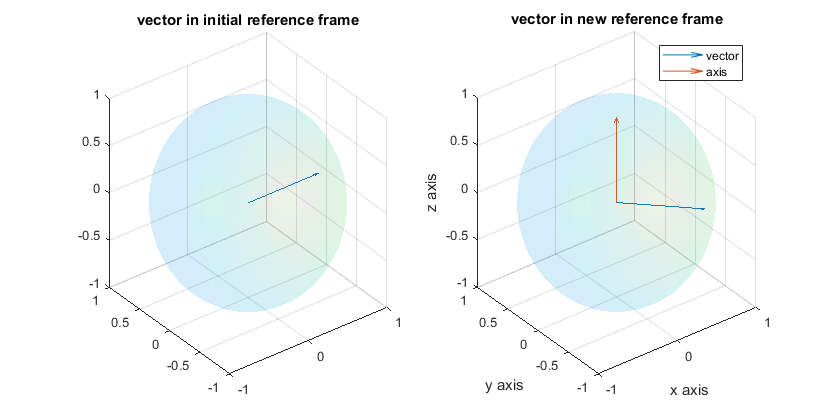
\includegraphics[width = 16cm]{./snap1.png}
\end{center}

\section*{Directory Tree}
\begin{flushleft}
\dirtree{%
.1 {./}.
.2 {README.md}.
.2 {driver.m}.
.2 {quatRotateDup.m}.
.2 {quatMult.m}.
.2 {quatTest.m}.
}
\end{flushleft}

\newpage
\section*{README.md}
\lstinputlisting[language=C]{README.md}

\newpage
\bibliography{references}

\end{document}
